% DIALS architecture, left-to-right version of figures/architecture.tex for the paper.
\documentclass[tikz,border=3pt]{standalone}
\usepackage{amsmath,amssymb}
\usepackage{fontawesome5}
\usetikzlibrary{arrows.meta,calc}
\definecolor{fzfill}{HTML}{E3EFFA}\definecolor{fzline}{HTML}{3B7FC4}
\definecolor{trfill}{HTML}{FDE6CF}\definecolor{trline}{HTML}{D9730D}
\definecolor{cC}{HTML}{7B4FB8}\definecolor{cL}{HTML}{1C9A8A}\definecolor{cG}{HTML}{3A8F3A}\definecolor{cS}{HTML}{C8372D}
\newcommand{\fire}{{\color{trline}\faFire}}
\newcommand{\snow}{{\color{fzline}\faSnowflake}}
\tikzset{
  arr/.style={-{Stealth[length=1.8mm]},line width=0.6pt,draw=black!70},
  bus/.style={line width=0.8pt,draw=black!70},
  frozen/.style={draw=fzline,fill=fzfill,line width=0.7pt,rounded corners=1.2pt},
  train/.style={draw=trline,fill=trfill,line width=0.8pt,rounded corners=2.5pt},
  tower/.style={draw=black!35,fill=black!2,line width=0.7pt,rounded corners=5pt},
  lab/.style={font=\small},
  tiny/.style={font=\scriptsize},
  op/.style={circle,draw=black!70,line width=0.7pt,minimum size=5mm,inner sep=0pt,fill=white},
}
% vertical score bar: centre x, centre y, colour (12 cells of 0.2 cm)
\newcommand{\vbar}[3]{%
  \foreach \v [count=\i] in {25,70,15,85,40,55,10,95,35,20,65,45}{
    \fill[#3!\v!white] ($(#1,#2)+(-0.15,{1.2-\i*0.2})$) rectangle ++(0.3,0.2);}
  \draw[black!60,line width=0.5pt] ($(#1,#2)+(-0.15,-1.2)$) rectangle ++(0.3,2.4);}

\begin{document}
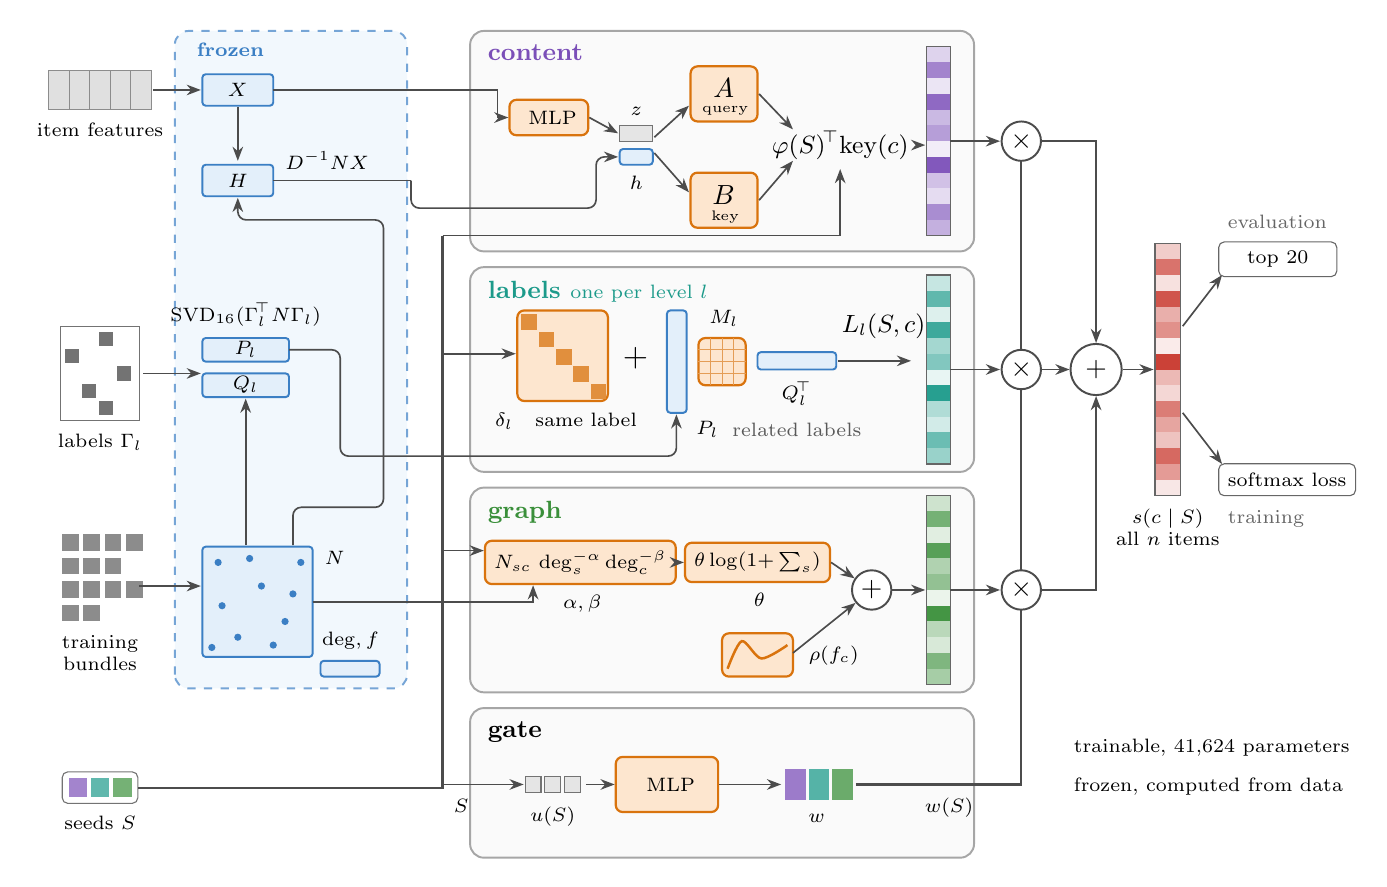
\begin{tikzpicture}[x=1cm,y=1cm]

% ============================================================ INPUTS (left)
% item features: a stack of feature rows
\foreach \k in {0,...,4}{\fill[black!12] (0.0+0.26*\k,8.35) rectangle ++(0.26,0.5);\draw[black!45] (0.0+0.26*\k,8.35) rectangle ++(0.26,0.5);}
\node[tiny,below,align=center] at (0.65,8.3) {item features};
% labels: an incidence pattern
\draw[black!55] (0.15,4.4) rectangle (1.15,5.6);
\foreach \r/\c in {0/2,1/0,2/3,3/1,4/2}{\fill[black!55] (0.2+0.22*\c,5.35-0.22*\r) rectangle ++(0.18,0.18);}
\node[tiny,below] at (0.65,4.35) {labels $\Gamma_l$};
% training bundles: rows of items
\foreach \row/\len in {0/4,1/3,2/4,3/2}{\foreach \k in {1,...,\len}{\fill[black!45] (-0.1+0.27*\k,2.75-0.3*\row) rectangle ++(0.21,0.21);}}
\node[tiny,below,align=center] at (0.65,1.8) {training\\bundles};
% seeds
\foreach \k/\c in {0/cC,1/cL,2/cG}{\fill[\c!70] (0.25+0.28*\k,-0.38) rectangle ++(0.24,0.24);}
\draw[black!55,rounded corners=2pt] (0.17,-0.46) rectangle (1.13,-0.06);
\node[tiny,below] at (0.65,-0.5) {seeds $S$};

% ============================================================ FROZEN DATA
\draw[fzline!70,dashed,fill=fzfill!45,rounded corners=5pt,line width=0.7pt] (1.6,1.0) rectangle (4.55,9.35);
\node[anchor=north west,font=\scriptsize\bfseries,text=fzline] at (1.65,9.32) {\snow\ frozen};
% X and H
\draw[frozen] (1.95,8.4) rectangle ++(0.9,0.4);\node[tiny] at (2.4,8.6) {$X$};
\draw[frozen] (1.95,7.25) rectangle ++(0.9,0.4);\node[tiny] at (2.4,7.45) {$H$};
\node[tiny,anchor=south west] at (2.88,7.47) {$D^{-1}NX$};
\draw[arr] (2.4,8.38) -- (2.4,7.7);
% P and Q
\draw[frozen] (1.95,5.15) rectangle ++(1.1,0.3);\node[tiny] at (2.5,5.3) {$P_l$};
\draw[frozen] (1.95,4.7) rectangle ++(1.1,0.3);\node[tiny] at (2.5,4.85) {$Q_l$};
\node[tiny,anchor=south] at (2.5,5.47) {SVD$_{16}(\Gamma_l^{\!\top}N\Gamma_l)$};
% N, deg, f
\draw[frozen] (1.95,1.4) rectangle ++(1.4,1.4);
\foreach \x/\y in {0.2/1.2,0.45/0.25,0.75/0.9,1.05/0.45,0.25/0.65,1.25/1.2,0.9/0.15,0.6/1.25,1.15/0.8,0.12/0.12}{\fill[fzline] (1.95+\x,1.4+\y) circle (1.3pt);}
\node[tiny,anchor=south west] at (3.38,2.45) {$N$};
\draw[frozen] (3.45,1.15) rectangle ++(0.75,0.2);\node[tiny,anchor=south] at (3.83,1.37) {$\deg,f$};
% how they are built
\draw[arr] (1.32,8.6) -- (1.93,8.6);
\draw[arr] (1.2,5.0) -- (1.93,5.0);
\draw[arr] (1.15,2.3) -- (1.93,2.3);
\draw[arr] (2.5,2.82) -- (2.5,4.68);           % N -> P, Q
\draw[arr,rounded corners=3pt] (3.1,2.82) -- (3.1,3.3) -- (4.25,3.3) -- (4.25,6.95) -- (2.4,6.95) -- (2.4,7.23); % N -> H

% ============================================================ SEED BUS
\draw[bus] (1.13,-0.26) -- (5.0,-0.26) -- (5.0,6.75);
\node[tiny,anchor=north west] at (5.02,-0.28) {$S$};

% ============================================================ TOWERS (bands)
\draw[tower] (5.35,6.55) rectangle (11.75,9.35);\node[font=\small\bfseries,text=cC,anchor=north west] at (5.45,9.3) {content};
\draw[tower] (5.35,3.75) rectangle (11.75,6.35);\node[font=\small\bfseries,text=cL,anchor=north west] at (5.45,6.3) {labels};
\node[tiny,text=cL,anchor=north west] at (6.5,6.25) {one per level $l$};
\draw[tower] (5.35,0.95) rectangle (11.75,3.55);\node[font=\small\bfseries,text=cG,anchor=north west] at (5.45,3.5) {graph};
\draw[tower] (5.35,-1.15) rectangle (11.75,0.75);\node[font=\small\bfseries,anchor=north west] at (5.45,0.7) {gate};

% ---------------- content
\node[train,minimum width=1.0cm,minimum height=0.45cm,font=\scriptsize] (mlp) at (6.35,8.25) {\fire\ MLP};
\draw[arr] (2.85,8.6) -- (5.7,8.6) -- (5.7,8.25) -- (mlp.west);                % X -> MLP
\draw[black!55,fill=black!10] (7.25,7.95) rectangle ++(0.42,0.2);\node[tiny,anchor=south] at (7.46,8.15) {$z$};
\draw[frozen] (7.25,7.65) rectangle ++(0.42,0.2);\node[tiny,anchor=north] at (7.46,7.63) {$h$};
\draw[arr] (mlp.east) -- (7.23,8.05);
\draw[line width=0.6pt,draw=black!70] (2.85,7.45) -- (4.6,7.45);
\draw[arr,rounded corners=3pt] (4.6,7.45) -- (4.6,7.1) -- (6.95,7.1) -- (6.95,7.75) -- (7.23,7.75);   % H -> h
\draw[train] (8.15,8.2) rectangle ++(0.85,0.7);\node at (8.57,8.62) {$A$};\node[font=\tiny] at (8.57,8.34) {\fire\,query};
\draw[train] (8.15,6.85) rectangle ++(0.85,0.7);\node at (8.57,7.27) {$B$};\node[font=\tiny] at (8.57,6.99) {\fire\,key};
\draw[arr] (7.69,8.0) -- (8.13,8.4);\draw[arr] (7.69,7.8) -- (8.13,7.3);
\node[lab] (cf) at (10.05,7.9) {$\varphi(S)^{\!\top}\mathrm{key}(c)$};
\draw[arr] (9.02,8.55) -- (9.45,8.1);\draw[arr] (9.02,7.2) -- (9.45,7.7);
\draw[arr] (5.0,6.75) -- (10.05,6.75) -- (cf.south);                         % S -> phi
\vbar{11.3}{7.95}{cC}\node[lab,anchor=south] at (11.3,9.15) {};
\draw[arr] (cf.east) ++(0,0) -- (11.13,7.9);

% ---------------- labels: diagonal + low rank
\draw[train] (5.95,4.65) rectangle ++(1.15,1.15);
\foreach \k in {0,...,4}{\fill[trline!80] (6.0+0.22*\k,5.55-0.22*\k) rectangle ++(0.2,0.2);}
\node[tiny,anchor=north] at (6.52,4.62) {\fire\ $\delta_l$\quad same label};
\node[font=\large] at (7.45,5.2) {$+$};
\draw[frozen] (7.85,4.5) rectangle ++(0.25,1.3);\node[tiny,anchor=north west] at (8.1,4.52) {$P_l$};
\draw[train] (8.25,4.85) rectangle ++(0.6,0.6);
\foreach \k in {0.15,0.3,0.45}{\draw[trline!70,line width=0.35pt] (8.25+\k,4.85) -- ++(0,0.6);\draw[trline!70,line width=0.35pt] (8.25,4.85+\k) -- ++(0.6,0);}
\node[tiny,anchor=south] at (8.55,5.47) {\fire\,$M_l$};
\draw[frozen] (9.0,5.05) rectangle ++(1.0,0.22);\node[tiny,anchor=north] at (9.5,5.02) {$Q_l^{\!\top}$};
\node[tiny,text=black!65,anchor=north] at (9.5,4.5) {related labels};
\draw[arr,rounded corners=3pt] (3.05,5.3) -- (3.7,5.3) -- (3.7,3.95) -- (7.97,3.95) -- (7.97,4.48);   % P, Q into the low-rank part
\node[lab] (lc) at (10.6,5.6) {$L_l(S,c)$};
\draw[arr] (10.02,5.16) -- (10.95,5.16);
\draw[arr] (5.0,5.25) -- (5.93,5.25);                                         % S -> labels
\vbar{11.3}{5.05}{cL}

% ---------------- graph
\node[train,minimum width=2.1cm,minimum height=0.55cm,font=\scriptsize] (deg) at (6.75,2.6) {$N_{sc}\,\deg_s^{-\alpha}\deg_c^{-\beta}$};
\node[tiny,anchor=north] at (deg.south) {\fire\,$\alpha,\beta$};
\node[train,minimum width=1.6cm,minimum height=0.5cm,font=\scriptsize] (damp) at (9.0,2.6) {$\theta\log(1{+}\textstyle\sum_s)$};
\node[tiny,anchor=north] at (damp.south) {\fire\,$\theta$};
\draw[arr] (deg) -- (damp);
\draw[train] (8.55,1.15) rectangle ++(0.9,0.55);
\draw[trline,line width=0.9pt] plot[smooth] coordinates {(8.62,1.25) (8.8,1.6) (9.05,1.38) (9.38,1.55)};
\node[tiny,anchor=west] at (9.48,1.42) {\fire\,$\rho(f_c)$};
\node[op] (gplus) at (10.45,2.25) {$+$};
\draw[arr] (damp.east) -- (gplus);\draw[arr] (9.45,1.45) -- (gplus);
\draw[arr] (3.35,2.1) -- (6.15,2.1) -- (6.15,2.31);   % N -> graph
\draw[arr] (5.0,2.75) -- (deg.west|-5.0,2.75);                                  % S -> graph
\vbar{11.3}{2.25}{cG}
\draw[arr] (gplus) -- (11.13,2.25);

% ---------------- gate
\foreach \k in {0,1,2}{\draw[black!55,fill=black!10] (6.05+0.25*\k,-0.32) rectangle ++(0.2,0.2);}
\node[tiny,anchor=north] at (6.4,-0.38) {$u(S)$};
\draw[arr] (5.0,-0.22) -- (6.03,-0.22);
\node[train,minimum width=1.3cm,minimum height=0.7cm,font=\scriptsize,align=center] (gmlp) at (7.85,-0.22) {\fire\ MLP};
\draw[arr] (6.82,-0.22) -- (gmlp);
\foreach \k/\c in {0/cC,1/cL,2/cG}{\fill[\c!75] (9.35+0.3*\k,-0.42) rectangle ++(0.26,0.4);}
\node[tiny,anchor=north] at (9.75,-0.47) {$w$};
\draw[arr] (gmlp) -- (9.3,-0.22);

% ============================================================ WEIGHTED SUM
\draw[bus] (10.25,-0.22) -- (12.35,-0.22) -- (12.35,7.95);
\node[tiny,anchor=north west] at (11.0,-0.27) {$w(S)$};
\foreach \y in {7.95,5.05,2.25}{\draw[arr] (11.45,\y) -- (12.08,\y);\node[op] at (12.35,\y) {$\times$};}
\node[op,minimum size=6.5mm,font=\normalsize] (sum) at (13.3,5.05) {$+$};
\draw[arr] (12.6,7.95) -- (13.3,7.95) -- (sum);\draw[arr] (12.6,5.05) -- (sum);\draw[arr] (12.6,2.25) -- (13.3,2.25) -- (sum);

% ============================================================ SCORE AND OUTPUT
\foreach \v [count=\i] in {25,70,15,85,40,55,10,95,35,20,65,45,30,75,50,12}{\fill[cS!\v!white] (14.05,{6.65-\i*0.2}) rectangle ++(0.32,0.2);}
\draw[black!60,line width=0.5pt] (14.05,3.45) rectangle ++(0.32,3.2);
\node[tiny,anchor=north,align=center] at (14.21,3.4) {$s(c\mid S)$\\all $n$ items};
\draw[arr] (sum) -- (14.03,5.05);
\draw[arr] (14.4,5.6) -- (14.9,6.25);\draw[arr] (14.4,4.5) -- (14.9,3.85);
\node[draw=black!60,rounded corners=2pt,tiny,minimum width=1.5cm,anchor=west] at (14.85,6.45) {top 20};
\node[tiny,text=black!60,anchor=south west] at (14.85,6.72) {evaluation};
\node[draw=black!60,rounded corners=2pt,tiny,minimum width=1.5cm,anchor=west] at (14.85,3.65) {softmax loss};
\node[tiny,text=black!60,anchor=north west] at (14.85,3.38) {training};

% ============================================================ LEGEND
\node[anchor=west,tiny] at (12.8,0.25) {\fire\ trainable, 41{,}624 parameters};
\node[anchor=west,tiny] at (12.8,-0.25) {\snow\ frozen, computed from data};
\end{tikzpicture}
\end{document}
